%% ISAE-SUPAERO report template for research projects 
%% V1.0
%% 2016/04/14
%% by Damien Roque
%% See http://personnel.isae.fr/damien-roque


%% This template is based on bare_conf.tex
%% V1.4b
%% 2015/08/26
%% by Michael Shell

%%*************************************************************************
%% Legal Notice:
%% This code is offered as-is without any warranty either expressed or
%% implied; without even the implied warranty of MERCHANTABILITY or
%% FITNESS FOR A PARTICULAR PURPOSE! 
%% User assumes all risk.
%% In no event shall the IEEE or any contributor to this code be liable for
%% any damages or losses, including, but not limited to, incidental,
%% consequential, or any other damages, resulting from the use or misuse
%% of any information contained here.
%%
%% All comments are the opinions of their respective authors and are not
%% necessarily endorsed by the IEEE.
%%
%% This work is distributed under the LaTeX Project Public License (LPPL)
%% ( http://www.latex-project.org/ ) version 1.3, and may be freely used,
%% distributed and modified. A copy of the LPPL, version 1.3, is included
%% in the base LaTeX documentation of all distributions of LaTeX released
%% 2003/12/01 or later.
%% Retain all contribution notices and credits.
%% ** Modified files should be clearly indicated as such, including  **
%% ** renaming them and changing author support contact information. **
%%*************************************************************************

\documentclass[conference]{IEEEtran}

\usepackage[utf8]{inputenc}
\usepackage{ifthen}
\usepackage{cite}
\usepackage[pdftex]{graphicx}
\graphicspath{{images/}}
\usepackage{tikz,filecontents}
\usetikzlibrary{shapes,arrows,shadings,patterns}
\usepackage{pgfplots}
\pgfplotsset{compat=newest}
\pgfplotsset{plot coordinates/math parser=false}
\newlength\figureheight
\newlength\figurewidth

\usepackage{amsfonts}
\usepackage[cmex10]{amsmath}
\usepackage{multirow}
\documentclass[a4paper,12pt]{article}
\usepackage[spanish]{babel}
\usepackage[latin1]{inputenc}
\usepackage[usenames]{color}

% Examples of several macros
\newcommand*{\SET}[1]{\ensuremath{\boldsymbol{#1}}}
\newcommand*{\VEC}[1]{\ensuremath{\boldsymbol{\mathrm{#1}}}}
\newcommand*{\FAM}[1]{\ensuremath{\mathrm{#1}}}
\newcommand*{\MAT}[1]{\ensuremath{\boldsymbol{\mathrm{#1}}}}
\newcommand*{\OP}[1]{\ensuremath{\mathrm{#1}}}
\newcommand*{\NORM}[1]{\ensuremath{\left\|#1\right\|}}
\newcommand*{\DPR}[2]{\ensuremath{\left \langle #1,#2 \right \rangle}}

\newtheorem{theorem}{Theorem}

\newcommand{\alert}[1]{\textcolor{red}{#1}}
\usepackage[caption=false,font=footnotesize]{subfig}
\usepackage{url}


% correct bad hyphenation here
\hyphenation{op-tical net-works semi-conduc-tor}


\begin{document}
%
% paper title
% Titles are generally capitalized except for words such as a, an, and, as,
% at, but, by, for, in, nor, of, on, or, the, to and up, which are usually
% not capitalized unless they are the first or last word of the title.
% Linebreaks \\ can be used within to get better formatting as desired.
% Do not put math or special symbols in the title.
\title{Flutter sensibility to semi-aeroelastic hinged wing parameters}

% for over three affiliations, or if they all won't fit within the width
% of the page, use this alternative format:
% 
\author{\IEEEauthorblockN{Carlos Nicol\'as Juarez\IEEEauthorrefmark{1},
Joseph Morlier\IEEEauthorrefmark{2}}
\IEEEauthorblockA{\IEEEauthorrefmark{1}Institut Supérieur de l'Aéronautique et de l'Espace (ISAE-SUPAERO), Université de Toulouse, 31055 Toulouse, FRANCE\\
Email: carlos.juarez@student.isae-supaero.fr}
\IEEEauthorblockA{\IEEEauthorrefmark{2}Institut Supérieur de l'Aéronautique et de l'Espace (ISAE-SUPAERO), Université de Toulouse, 31055 Toulouse, FRANCE\\
Email: joseph.morlier@isae-supaero.fr}
}


%\IEEEspecialpapernotice{(Bibliography report)}
\IEEEspecialpapernotice{(Final report)}


% make the title area
\maketitle

% As a general rule, do not put math, special symbols or citations
% in the abstract
\textcolor{blue}{\textbf{BLUE MEANS NEW MATERIAL}}


\begin{abstract}
The benefits of high aspect ratio wings in lift-induced drag are well known. However, this solution has well-defined limits imposed by airport regulation and increasing loads. The introduction of a hinged wingtip is a possible solution for both problems. The aim of this research is to study the influence of hinge parameters on the flutter performance of the wing.
\end{abstract}

\IEEEpeerreviewmaketitle

\section*{Nomenclature}
\subsection*{Symbols}
\begin{tabular}{l l}
$k_{hinge}$&    Hinge stiffness\\
$y_{hinge}$&    Hinge position\\
$\Lambda$&      Flare angle\\
$\theta$ &      Winglet rotation angle\\
$M_{hinge}$&    Hinge moment\\
$\textbf{q}$&   Modal amplitudes\\
$\textbf{M}$&   Mass matrix\\
$\textbf{C}$&   Damping matrix\\
$\textbf{K}$&   Stiffness matrix\\
$q_{\infty}$&   Dynamic pressure\\
\end{tabular}

\subsection*{Abbreviations}

\begin{tabular}{l l}
HAR&    High aspect ratio\\
SAH&    Semi-aeroelastic hinge\\
DLM&    Doublet lattice method\\
WRBM&   Wing root bending moment\\
MAC&    Mean aerodynamic chord\\
HTP&    Horizontal tail plane\\
VTP&    Vertical tail plane\\
GUI&    Graphic user interface\\
DoF&    Degrees of freedom\\
\end{tabular}



\section{Introduction}
\label{sec:problem-statement}

One of the most efficient strategies to reduce aerodynamic drag is to attack the lift-induced drag given that it contributes approximately 40\% of the overall drag. Induced drag is created at the tips of the wings where the high pressure air from beneath the wing comes up over the wing tips into the low pressure zone. This meeting place of different air pressures becomes a turbulent area creating induced drag. High aspect ratio (HAR) wings reduce considerably this effect, since the lift-induced drag is proportional to the reciprocal of the wingspan squared. Despite this great advantage, HAR wings are limited by two main issues: On one hand, maximum aircraft dimensions allowed in airports, and on the other hand the increase in bending moments along the wing.

In the last years, some attempts were made in order to increase civil aircraft wingspan; for example, the implementation of a folding wingtip in the Boeing 777X which enables the reduction of the wingspan when grounded in order to respect airport regulations.

In this research, an alternative design is studied, which is a potential solution for both problems mentioned. The main idea consists in introducing a hinge (with a certain stiffness) in order to allow the wing tips to rotate as can be seen in fig. 1. Such a concept is called semi-aeroelastic hinge (SAH) \cite{Castrichini2016,Castrichini2020}. 

\begin{figure}[htp]
  \centering
  \setlength\figureheight{5cm}
  \setlength\figurewidth{6cm}
  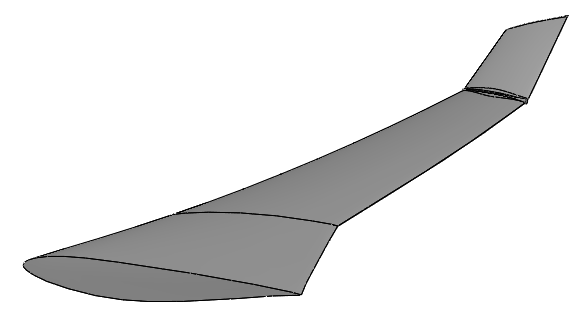
\includegraphics[width=200pt]{images/HingedWing.png}
  \caption{Geometric model of a SAH}
  \label{fig:my-figure}
\end{figure}

Significant progress in this field is the Airbus project AlbatrosONE, which consists of a small scale demonstrator, and, so far, has presented optimistic results from wind tunnel tests and from the first flight tests \cite{wilson2019small}.

This solution has shown itself to be quite favourable when looking for load alleviation. Previous studies found between 10\% and 20\% reduction in the wing root bending moment (WRBM) depending on the design chosen and the conditions studied. Despite these benefits, the hinge presence may introduce instabilities to the aircraft, generating undesired effects like flutter.

This research looks to analyse flutter, which is a dangerous aeroelastic phenomenon that arises from an unfavourable coupling between aerodynamic, elastic and inertial forces. This instability produces large displacements that can generate severe damage or even destruction of the aircraft and hence, it must be taken into account from a preliminary design phase. The idea in this work is to better understand how flutter is affected by hinge parameters.



\section{Problem statement}
\label{sec:problem-statement}

The aim of this work is to represent this new design solution by using low-fidelity models and then to modify the main parameters concerning the hinge in order to see how they affect flutter speed.

The framework to be used for this work is NeoCASS, a free suite of Matlab modules that combines state of the art computational, analytical and semi-empirical methods to run aero-structural analysis of a design layout at conceptual design stage. It works with NASTRAN derived formats \cite{cavagna2011neocass}.

One of the challenges that arise in order to work with this framework is that even if non-conventional designs are supported, there is no option to model a semi-rigid hinge, therefore, a modification in the modelling process is needed to include it.

Several combinations of the hinge parameters will be done, computing flutter performance for each case in order to extract valuable information about its sensibility. An appropriate range of values will be defined for each parameters taking into account possible design solutions.

The idea is to choose those parameters that are most related to the hinge presence.

It is known that the hinge stiffness $k_{hinge}$ is a significant parameter. Previous works \cite{Wilson2014,Castrichini2016}show that a zero stiffness hinge is highly effective for load alleviation. However, this may generate instability and flutter.

Another important parameter is the hinge position $y_{hinge}$. Previous results indicate that moving the hinge inboard may produce a strong stabilising effect on the flutter mechanisms \cite{Wilson2014}.

Finally the orientation of the hinge line relative to the airflow (flare angle $\Lambda$) is a key parameter to enable successful load alleviation. When the hinge line is rotated outboard of the streamline, folding the wingtip up introduces a decrease in the local angle of attack; such an effect provides a means to reduce the loads acting on the wing, leading to the possibility of achieving a wing tip extension with limited or even minimal impact on wing weight. Although this angle may also have an effect over the flutter speed this parameter will not be considered due to model limitations \cite{Castrichini2020,Wilson2014}.



\section{Aeroelastic model}
\label{sec:aeroelastic-model}
A low-fidelity model is used in order to obtain results without high computational cost but still accurate enough to obtain qualitative information. The main modelling is done in AcBuilder \cite{acbuilderfurther}, a graphical editor where a conceptual design of the aircraft is done and also, the XML file requested by NeoCASS is generated.

\subsection{Aircraft modelling}
\textcolor{blue}{Three models were used: First, a generic short-range airplane, comparable in its dimensions with the A320 or the 737 families, where the wing span (including the wingtip with no deflection angle) was increased 10\% from the AcBuilder default value. Then, a similar model where the wing span was increased 25\% and finally a long-range aircraft based on the Boeing 747-100 which is already available as an example in NeoCASS, therefore, only the hinge modelling was needed. This article is focused on the results obtained from the last model as they were clearer. Main geometric specifications values are shown in table 1.}

\begin{table}[t]
\begin{center}
\begin{tabular}{| l | r |}
\hline
Overall length & $68.5 \; m$ \\ \hline
Wing span & $59.64 \;m$ \\ \hline
Wing surface & $551 \;m^2$ \\\hline
MAC & $ \;10.0695 m$\\\hline
Airfoil &  N64A410\\ \hline
HTP surface & $135 m^2$\\\hline
VTP surface & $77.11 m^2$\\
\hline 
\end{tabular}
\caption{Geometric specifications}
\label{tab:fruta}
\end{center}
\end{table}

The aircraft model as displayed in AcBuilder graphic user interface (GUI) is shown in figure 2.

\begin{figure}[htp]
  \centering
  \setlength\figureheight{5cm}
  \setlength\figurewidth{7cm}
  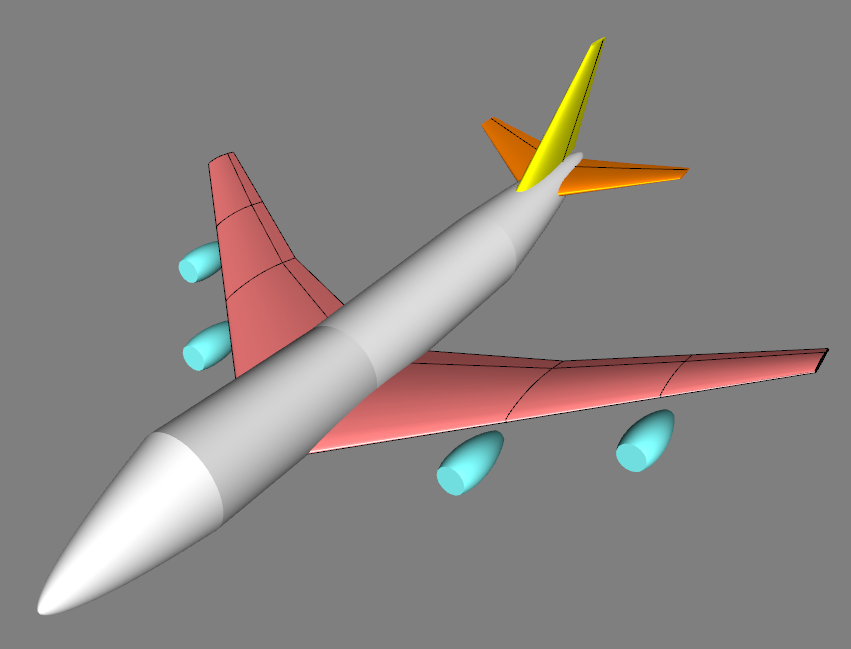
\includegraphics[width=225pt]{images/AircraftModel.png}
  \caption{Aircraft model}
  \label{fig:my-figure}
\end{figure}

\subsection{Structural modelling}
The structure was modelled using linear beam elements, discretizing each semi wing in $15$ elements. As a hinge definition is not supported by the AdBuilder GUI, a modification in the geometric file was needed. Thus the hinge was modelled by constraining two coincident nodes, one belonging to the main airframe and the other to the wing-tip, to have the same translations but free to have different relative rotations with respect to the hinge axis. This was done using CELAS, which is a zero-length Nastran elements used to model springs.

The implementation of CELAS elements is shown in figure 3, where a certain stiffness (in this case $k_{hinge} = 1e6 \frac{Nm}{rad}$) is given to the hinge rotation axis while the rest of the DoF are constrained with high stiffness values. \textcolor{blue}{In the figure example the spring element connect the node $2015$ with the node $2015555$ which is an intermediate node between the nodes $2015$ and $2016$ and it is coincident with the node $2015$.}

\begin{figure}[htp]
  \centering
  \setlength\figureheight{5cm}
  \setlength\figurewidth{7cm}
  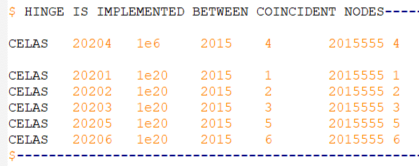
\includegraphics[width=225pt]{images/NastranHinge.png}
  \caption{CELAS elements implementation}
  \label{fig:my-figure}
\end{figure}

\textcolor{blue}{Previous works have shown that the wingtip mass have a certain influence in the flutter performance \cite{Castrichini2016}. In fact, for values lower than 300 kg, the sensitivity of the flutter speed with respect to the spring stiffness was negligible. Therefore, in order to analyze the hinge stiffness influence, concentrated masses were added to the wingtips using CONM2 Nastran elements. Their implementation is shown in figure 4.}

\begin{figure}[htp]
  \centering
  \setlength\figureheight{5cm}
  \setlength\figurewidth{7cm}
  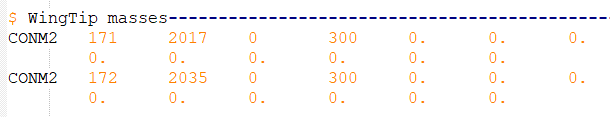
\includegraphics[width=225pt]{images/NastranCONM2.png}
  \caption{CONM2 elements implementation}
  \label{fig:my-figure}
\end{figure}

The structural model and discretization is shown in figure 5.

\begin{figure}[htp]
  \centering
  \setlength\figureheight{5cm}
  \setlength\figurewidth{7cm}
  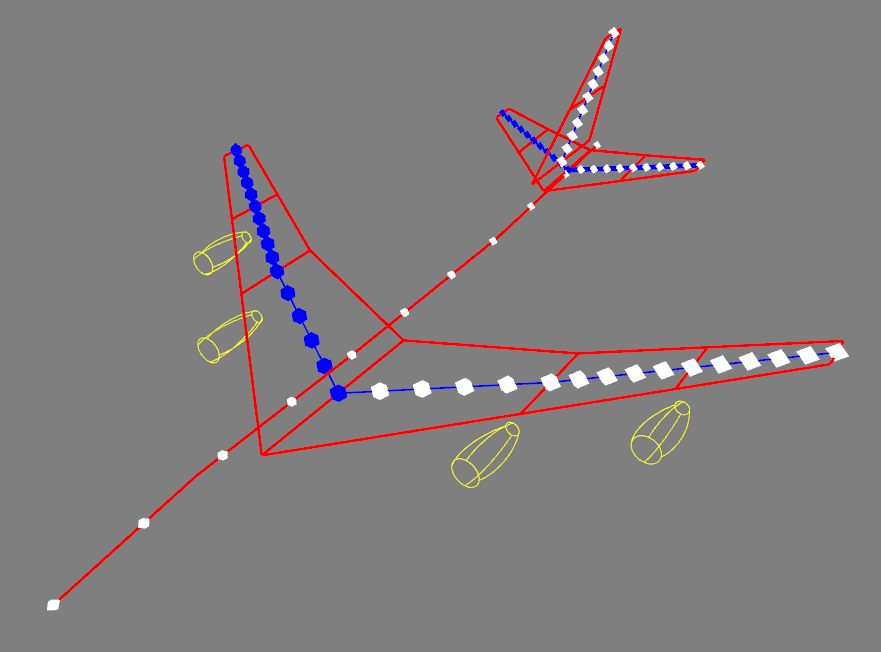
\includegraphics[width=225pt]{images/StructuralModel.png}
  \caption{Structural model}
  \label{fig:my-figure}
\end{figure}

\subsection{Aerodynamic modelling}
In order to compute the unsteady loads that are needed for the flutter computation NeoCASS applies the Doublet lattice method (DLM). This is a method based on aerodynamic potential theory, where each of the interfering surfaces is divided into small trapezoidal lifting elements (panels) such that the panels are arranged in strips parallel to the free stream with surface edges, fold lines, and hinge lines lying on box boundaries. The unknown lifting pressures are assumed to be concentrated uniformly across the one-quarter chord line of each box. There is one control point per box, centred span-wise on the three-quarter chord line of the box, and the surface boundary condition is satisfied at each of these points.

The implemented aerodynamic model has 14 span-wise divisions and 7 chord-wise divisions and it is shown in figure 6.

\begin{figure}[htp]
  \centering
  \setlength\figureheight{5cm}
  \setlength\figurewidth{7cm}
  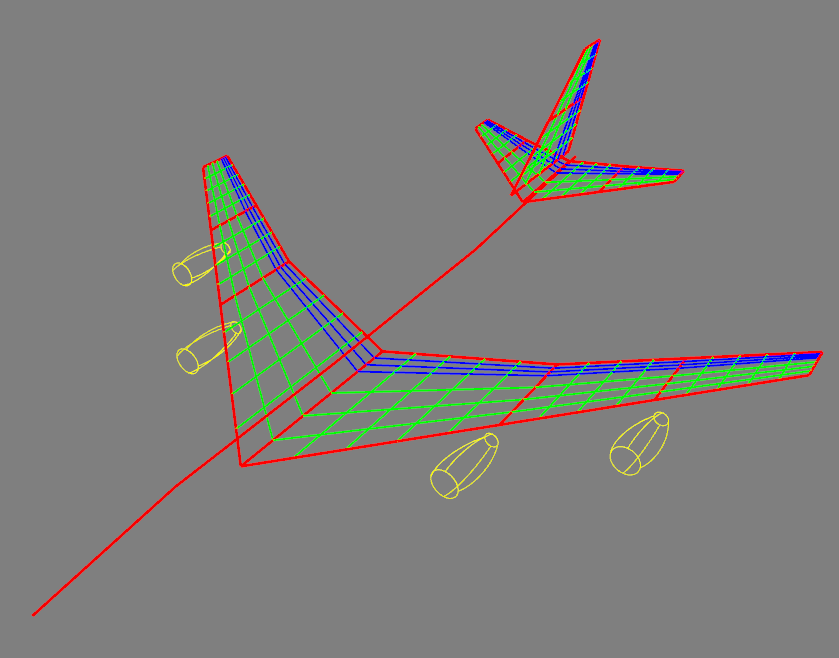
\includegraphics[width=225pt]{images/AeroModel.png}
  \caption{Aerodynamic model}
  \label{fig:my-figure}
\end{figure}



\section{Analyzed parameters}

\textcolor{blue}{In order to understand the hinge behaviour, two of the main parameters related to its presence were considered: the hinge stiffness and the hinge position.}

\subsection{Hinge stiffness}
\textcolor{blue}{The hinge is modelled as a rotational spring, which has a certain stiffness called $k_{hinge}$. When the winglet is deflected, the spring produces a moment proportional to the angle of rotation $\theta$:}

\begin{equation}
    M_{hinge} = k_{hinge}[\frac{Nm}{rad}] \times \theta
\end{equation}

\textcolor{blue}{Based on previous works, the chosen stiffness values are: }

\begin{itemize}
    \item $k_{hinge} = 1e3$
    \item $k_{hinge} = 1e4$
    \item $k_{hinge} = 5e4$
    \item $k_{hinge} = 1e5$
    \item $k_{hinge} = 5e5$
    \item $k_{hinge} = 1e6$
    \item $k_{hinge} = 5e6$
    \item $k_{hinge} = 1e7$
    \item $k_{hinge} = 5e7$
    \item $k_{hinge} = 1e8$
\end{itemize}

\textcolor{blue}{Also, the conventional case without hinge was considered for the comparison of results.}

\subsection{Hinge position}
\textcolor{blue}{The hinge position is defined as the ratio between the coordinate of the node where the hinge is placed and the wing span. The range of  selected values for this analysis is the following:}

\begin{itemize}
    \item $y_{hinge} = 0.67$
    \item $y_{hinge} = 0.72$
    \item $y_{hinge} = 0.78$
    \item $y_{hinge} = 0.83$
\end{itemize}

\textcolor{blue}{The identification of these nodes in the Nastran geometric file can be seen in figure 7.}

\begin{figure}[htp]
  \centering
  \setlength\figureheight{5cm}
  \setlength\figurewidth{6cm}
  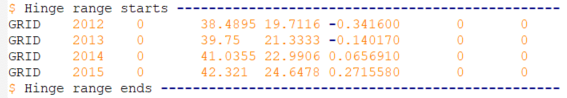
\includegraphics[width=250pt]{images/HingeRange.png}
  \caption{Hinge range in the geometric file}
  \label{fig:my-figure}
\end{figure}


\section{Modal analysis}
\textcolor{blue}{Modal analysis, or the mode-superposition method, is a linear dynamic-response procedure which evaluates and superimposes free-vibration mode shapes to characterize displacement patterns. The purpose of a modal analysis is to find the shapes and frequencies at which the structure will amplify the effect of a load.}

\textcolor{blue}{In order to compute flutter, modal analysis is needed for each hinge configuration. In the NeoCASS GUI this analysis can be easily set up.}

\textcolor{blue}{For this work 20 modes were computed, where the first 6 modes correspond to the rigid modes of the plane. The range of frequencies is set up from $0\;[Hz]$ to $50\;[Hz]$ which is large enough to include the first 20 modes. The configuration of the analysis in the NeoCASS GUI is shown in figure 8.}

\begin{figure}[htp]
  \centering
  \setlength\figureheight{5cm}
  \setlength\figurewidth{6cm}
  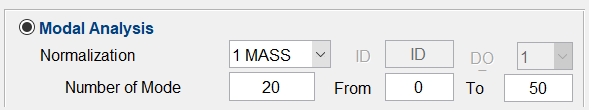
\includegraphics[width=250pt]{images/ModalGUI.png}
  \caption{Modal analysis set up}
  \label{fig:my-figure}
\end{figure}


\section{Flutter analysis}
\textcolor{blue}{The flutter analysis technique implemented in NeoCASS is based on a well-consolidated continuation form.
Adopting the classic assumptions based on assumed structural shapes, the availability of an aerodynamic
transfer matrix $\textbf{H}_{am}$ and the Laplace domain $s$, the flutter problem reads\cite{cavagna2011aeroelastic}:}

\begin{equation}
    (s^2 \textbf{M} + s \textbf{C} + \textbf{K} - q_{\infty} \textbf{H}_{am}(p,M_\infty))\textbf{q}=\textbf{0}
\end{equation}

\textcolor{blue}{Where $\textbf{q}$, $\textbf{M}$, $\textbf{C}$, $\textbf{K}$ are respectively modal amplitudes, mass, damping, and stiffness matrices, and $q_\infty$ is the dynamic pressure. Eq.(2) represents a complex eigenvalue problem and the method adopted for the solution is the one proposed in \cite{cardani1978continuation}.}

\textcolor{blue}{For all the different combinations of the studied parameters the Mach number was fixed to $M = 0.5$. And the density was fixed to a standard value $\rho = 1.225 [\frac{kg}{m^3}]$.}

\textcolor{blue}{The 20 computed modes were considered for the modal base. On the other hand, after considering first results, the study of flutter instability was focused on the firs non-rigid modes, i.e. modes 7 and 8.}

\textcolor{blue}{With respect to the reduced frequencies, eight values were chosen as they can be seen in figure 9.}

\begin{figure}[htp]
  \centering
  \setlength\figureheight{5cm}
  \setlength\figurewidth{6cm}
  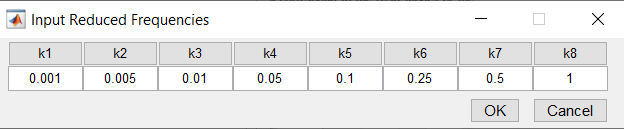
\includegraphics[width=250pt]{images/ReducedFreqGUI.png}
  \caption{Modal analysis set up}
  \label{fig:my-figure}
\end{figure}

\textcolor{blue}{The configuration of the analysis in the NeoCASS GUI is shown in figure 10.}

\begin{figure}[htp]
  \centering
  \setlength\figureheight{5cm}
  \setlength\figurewidth{6cm}
  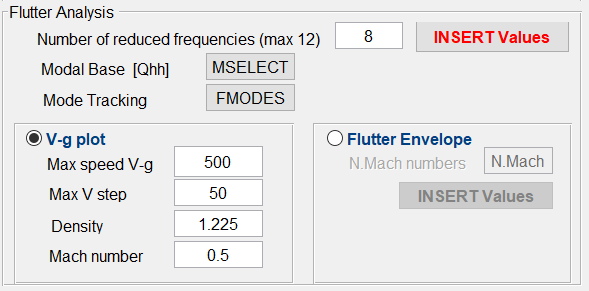
\includegraphics[width=250pt]{images/FlutterGUI.png}
  \caption{Modal analysis set up}
  \label{fig:my-figure}
\end{figure}


\section{Results}

\subsection{Modes}  
\subsection{Hinge stiffness influence}
\subsection{Hinge position influence}



\section{Conclusions}



\section{Future work}



% Optional section
\section*{Acknowledgment}
I would like to thank Dr. Morlier for the support during the investigation and most of all for giving me the opportunity to work on this fascinating subject.

\bibliographystyle{plain}
\bibliography{references}

\end{document}


